\apendice{Planificación}

\section{Introducción}
Para llevar a cabo este proyecto vamos a aplicar una metodología llamada \textit{Scrum}. \textit{Scrum} es una metodología de desarrollo software ágil, es decir, durante cada \textit{sprint}\footnote{\textit{Sprint}: es el período en el cual se lleva a cabo el trabajo en sí~\cite{wiki:scrum}.}, generalmente cada semana, se asignarán unas determinadas tareas a cumplimentar, con un producto como consecuencia de estas tareas. Al final de cada \textit{sprint} se realizará una reunión junto a los tutores para validar los avances realizados y determinar las tareas a realizar durante el siguiente \textit{sprint}.

Además, toda la comunicación se realizará a través de las \url{https://github.com/jasag/Phytoliths-recognition-system}{issues} de \textit{GitHub}.

\section{Planificación temporal}

En esta sección podremos ver la planificación del proyecto subdividida en \textit{sprints}, como previamente comentaba. En cada uno de los sprints se detalla las tareas a realizar, algunos detalles descriptivos y un gráfico \textit{burndown}.

% \section{Estudio previo}

\subsection{\textit{Sprint} 0}
Estas son las tareas a realizar durante este \textit{sprint} 0:

\begin{itemize}
	\item Probar \LaTeX.
	\item Gestor de tareas/versiones: \textit{Github} y \textit{Zenhub}.
	\item Instalar \textit{Anaconda} y \textit{Jupyter}.
	\item Leer los artículos propuestos por los tutores.
	\item Comenzar a probar algunos algoritmos de binarización.
\end{itemize}

Como se puede ver las tareas a realizar son básicas, puesto que es el \textit{sprint} 0 y es un \textit{sprint} de mera adaptación al entorno de trabajo. La única tarea que supone un esfuerzo de comprensión mayor es la lectura de los artículos propuestos sobre trabajos relacionados o con una problemática similar a la nuestra. A continuación, en la figura \ref{fig:A.1.1}, se muestra el diagrama \textit{burndown} de este \textit{sprint}. 

\begin{figure}
\centering
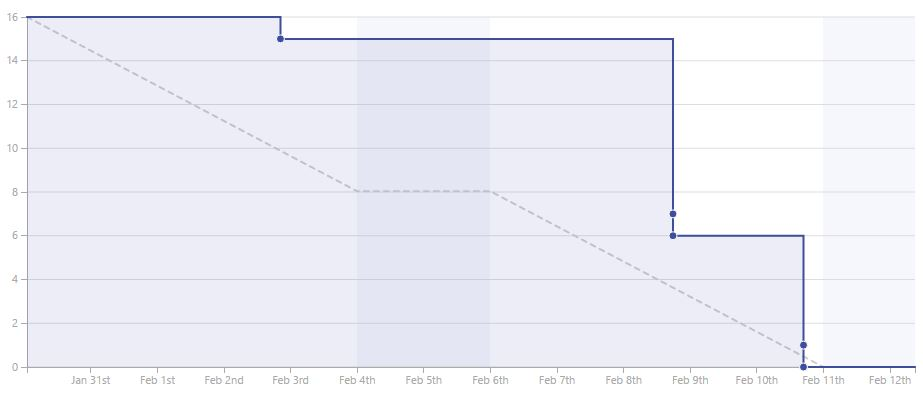
\includegraphics[width=0.99\textwidth]{sprint_0}
\caption{Burndown del \textit{sprint} 0}
\label{fig:A.1.1}
\end{figure}

\subsection{\textit{Sprint} 1}
Estas son las tareas a realizar durante esta \textit{sprint} 1:

\begin{itemize}
	\item Documentar lo realizado durante el \textit{sprint} 0.
	\item Documentar lo que se irá realizando durante este \textit{sprint} 1.
	\item Continuar probando con algoritmos de procesamiento de imágenes.
	\item Probar una aproximación con clasificadores al problema.
\end{itemize}

Puesto que en el \textit{sprint} anterior no se documentó lo realizado, durante éste se pretende documentar todo lo realizado durante el \textit{sprint} anterior y éste. Además de continuar probando con algoritmos de procesamiento de imágenes y comenzar a probar con la aproximación al problema mediante clasificadores.

En este \textit{sprint} me vi desbordado de trabajo debido a la subestimación del esfuerzo a empeñar en las distintas tareas. No siendo capaz de comenzar a probar una aproximación con clasificadores. Por ello la tarea <<Probar una aproximación con clasificadores al problema>> se vio movida al siguiente \textit{sprint}. 

A continuación, en la figura \ref{fig:A.1.2}, se muestra el diagrama \textit{burndown} de este \textit{sprint}. El cual tiene dicho aspecto debido a que muchas de las tareas se trabajaron de manera paralela, no siendo acabadas hasta el final del \textit{sprint}. Y, además, algunas de las tareas no fueron cerradas cuando se debió, aspecto que se corregirá en los siguientes \textit{sprints}.

\begin{figure}
\centering
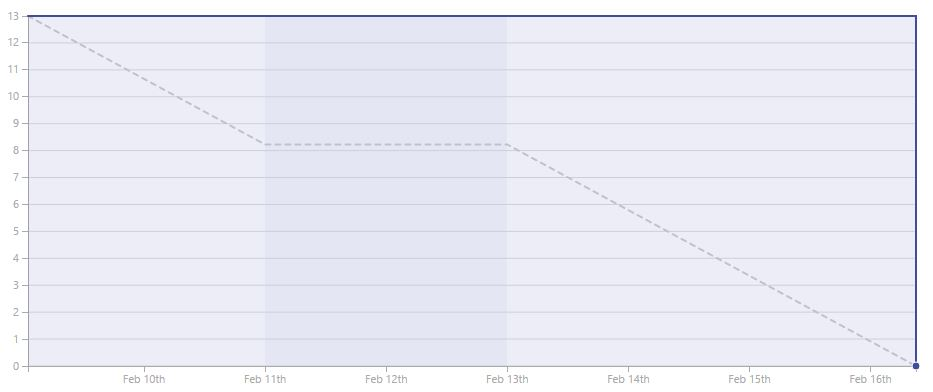
\includegraphics[width=0.99\textwidth]{sprint_1}
\caption{Burndown del \textit{sprint} 1}
\label{fig:A.1.2}
\end{figure}

\subsection{\textit{Sprint} 2}
Estas son las tareas a realizar durante este \textit{sprint} 2:

\begin{itemize}
	\item Probar una aproximación con clasificadores al problema.
	\item Aplicación del método <<Non-maximum suppression>> sobre el clasificado.
\end{itemize}

Puesto que la aproximación mediante reconocimiento de imágenes no reflejaba unos resultados muy positivos, durante la reunión mantenida con los tutores se decidió el uso de una técnica distinta. Nos referimos a la utilización  de un clasificador, junto a un descriptor visual.

Debido a que todavía no se poseían suficientes imágenes para el estudio del problema mediante esta técnica, lo que se decidió es aplicarla sobre otro problema de características similares, como es el reconocimiento de caras en imágenes. Con unos resultados bastante positivos debido a distintos razonamientos explicados en la Memoria, sección de Aspectos relevantes del proyecto.

A continuación, en la figura \ref{fig:A.1.3}, se muestra el diagrama \textit{burndown} de este \textit{sprint}.

\begin{figure}
\centering
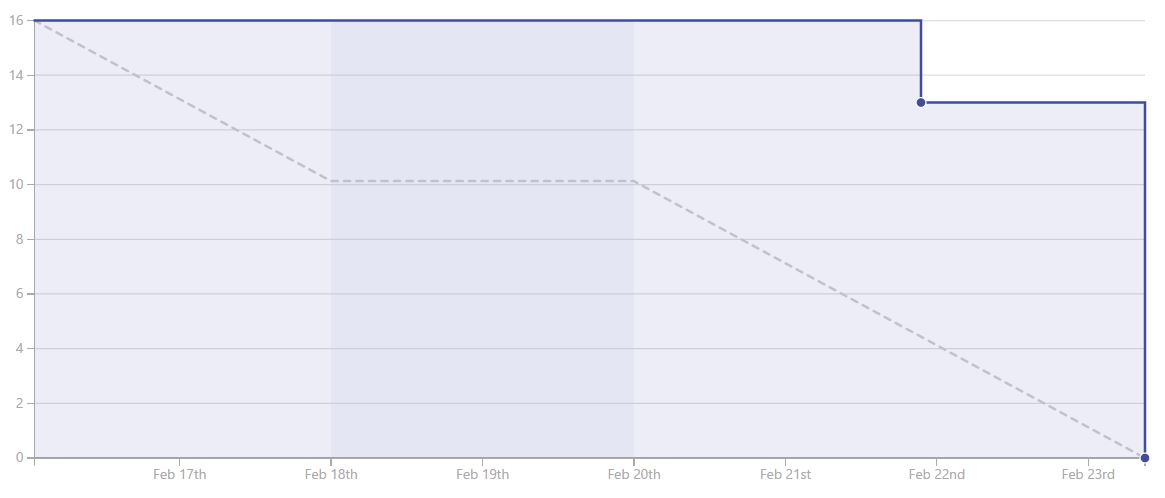
\includegraphics[width=0.99\textwidth]{sprint_2}
\caption{Burndown del \textit{sprint} 2}
\label{fig:A.1.3}
\end{figure}

\subsection{\textit{Sprint} 3}
Estas son las tareas a realizar durante este \textit{sprint} 3:

\begin{itemize}
	\item Reorganizar los \textit{Jupyter Notebooks}.
	\item Probar distintos clasificadores y métricas.
	\item Enviar fotos rotadas al clasificador.
\end{itemize}

Durante este \textit{sprint}, primero, se reorganizó la estructura del proyecto. Aportando mucho más orden y claridad a nuestro proyecto. Después, se introdujeron múltiples clasificadores y métricas, los cuales introduciré en mayor medida en la memoria, como \textit{Random Forest}~\cite{randomforest} o \textit{Gradient tree boosting}~\cite{gradientboosting}. Por último, se enviaron imágenes rotadas al clasificador, con el fin de poder analizar una posible problemática.

A continuación, en la figura \ref{fig:A.1.4}, se muestra el diagrama \textit{burndown} de este \textit{sprint}.

\begin{figure}
\centering
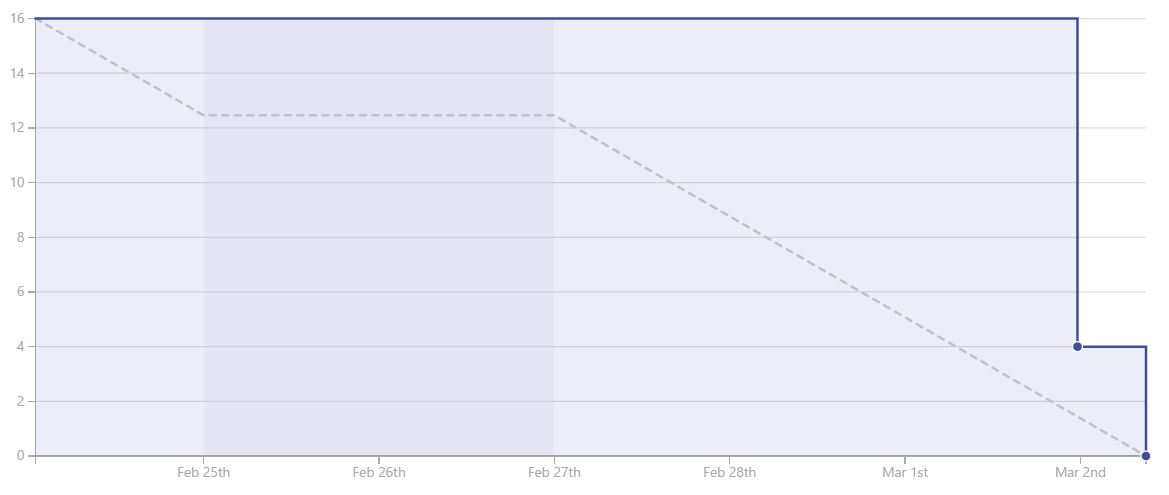
\includegraphics[width=0.99\textwidth]{sprint_3}
\caption{Burndown del \textit{sprint} 3}
\label{fig:A.1.4}
\end{figure}

\subsection{\textit{Sprint} 4}
Estas son las tareas a realizar durante este \textit{sprint} 4:

\begin{itemize}
	\item Implementación de \textit{Data Augmentation} en nuestro conjunto de entrenamiento.
	\item Implementación de controles de usuario.
\end{itemize}

Durante este \textit{sprint} se aplicó en nuestro conjunto de entrenamiento la técnica \textit{Data augmentation}. Esta técnica nos permitió aumentar el tamaño de nuestro conjunto de entrenamiento enormemente. 

Además, se realizó un \textit{notebook}\footnote{Siempre que nos referimos a un \textit{notebook}, a lo que nos referimos es a un \textit{Jupyter Notebook}}, con controles de usuario, los cuales nos permiten escoger entre clasificadores, imágenes y probabilidades. Permitiendo la continua interacción entre el usuario y la clasificación de una imagen, sin la necesidad de modificar el código por parte del usuario del notebook para cambiar entre las distintas opciones.

A continuación, en la figura \ref{fig:A.1.5}, se muestra el diagrama \textit{burndown} de este \textit{sprint}.

\begin{figure}
\centering
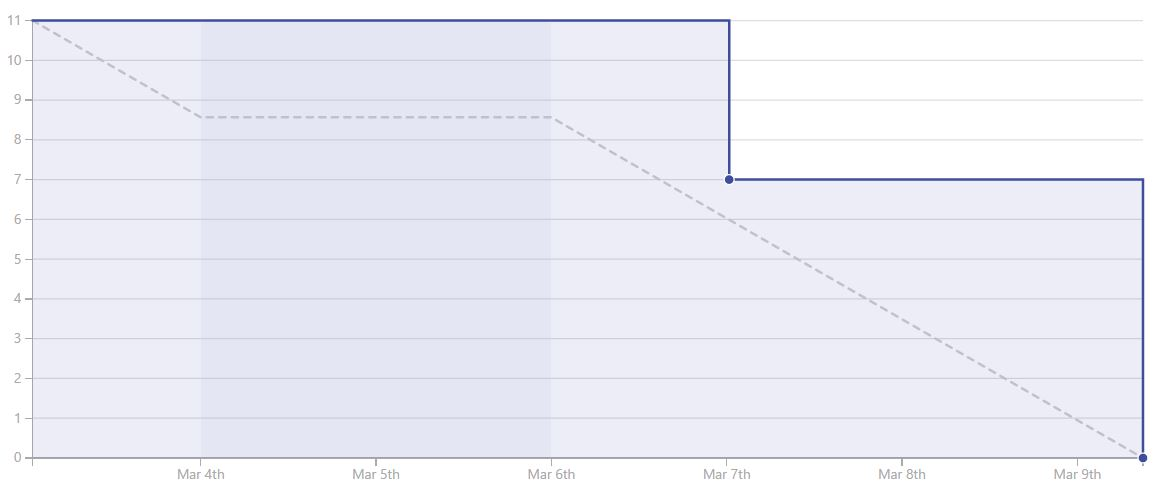
\includegraphics[width=0.99\textwidth]{sprint_4}
\caption{Burndown del \textit{sprint} 4}
\label{fig:A.1.5}
\end{figure}


\subsection{\textit{Sprint} 5}
Estas son las tareas a realizar durante este \textit{sprint} 5:

\begin{itemize}
	\item Implementar un \textit{file chooser} 
	\item Añadir más clasificadores.
	\item Correciones en la documentación.
	\item Estudiar como implementar un etiquetador de imágenes.
\end{itemize}

Durante este \textit{sprint} se añadieron los clasificadores que deseábamos, es decir, un clasificador bayesiano y un clasificador mediante regresión logística. Además, se añadió un \textit{file chooser} que nos permitiría, desde ese momento, escoger la imagen que deseemos dentro de nuestro sistema operativo. En cuanto a la documentación, se corrigió toda la  realizada hasta ese momento. Y, por último, se hizo un estudio básico sobre como implementar un etiquetador de imágenes mediante un \textit{Widget} de \textit{Python}. Aunque, esta última tarea no tuviese ningún producto resultante en este \textit{sprint}.

A continuación, en la figura \ref{fig:A.1.6}, se muestra el diagrama \textit{burndown} de este \textit{sprint}.

\begin{figure}
\centering
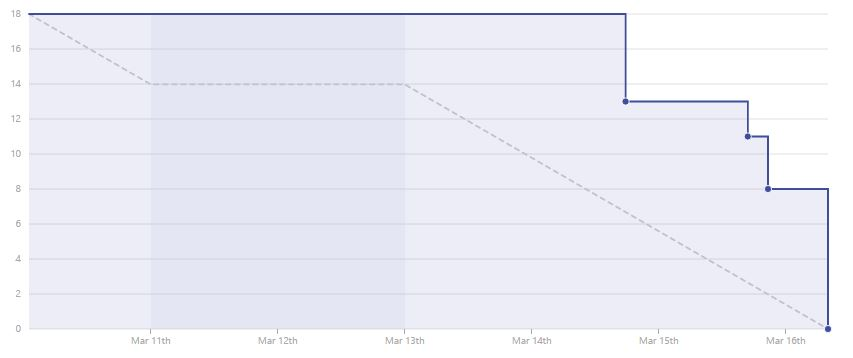
\includegraphics[width=0.99\textwidth]{sprint_5}
\caption{Burndown del \textit{sprint} 5}
\label{fig:A.1.6}
\end{figure}

\subsection{\textit{Sprint} 6}
Estas son las tareas a realizar durante este \textit{sprint} 6:

\begin{itemize}
	\item Estudiar los \textit{Widgets} personalizados de \textit{Jupyter Notebook} e \textit{Ipython}.
\end{itemize}

Aunque este \textit{sprint} se encuentre compuesto por una única tarea, no era menos complejo por ello. El objetivo de este \textit{sprint} era obtener un \textit{Widget} capaz de etiquetar imágenes. Pero en la realización de este se encontraron multiples problemas. Obteniendo como producto resultante tres posibles alternativas con aspectos a corregir.

Por lo tanto, en la figura \ref{fig:A.1.7} mostramos el diagrama \textit{burndown}, poco esclarecedor, de este \textit{sprint}.

\begin{figure}
\centering
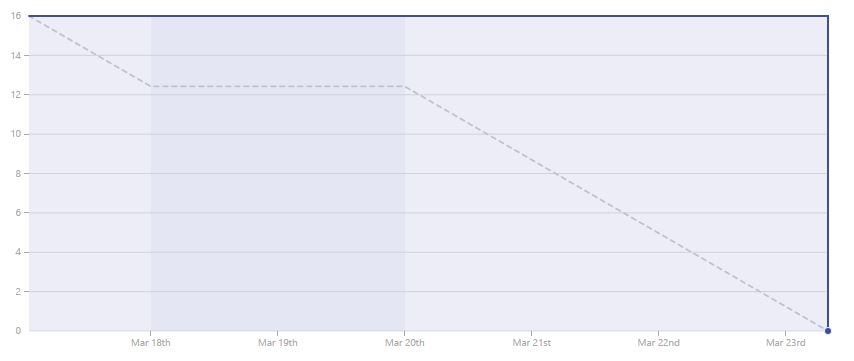
\includegraphics[width=0.99\textwidth]{sprint_6}
\caption{Burndown del \textit{sprint} 6}
\label{fig:A.1.7}
\end{figure}



\subsection{\textit{Sprint} 7}
Estas son las tareas a realizar durante este \textit{sprint} 7:

\begin{itemize}
	\item Estudiar \textit{Bag of Words}.
	\item Añadir mayor parametrización al \textit{Jupyter Notebook UI}.
	\item Corregir \textit{bugs} del Widget previamente implementado.
\end{itemize}

Durante este \textit{sprint} se consiguió, en primer lugar, corregir una de las alternativas del etiquetador de imágenes, o \textit{Widget}, desarrolladas durante el \textit{sprint} anterior. Además, se corrigieron y añadieron múltiples parámetros en el \textit{Jupyter Notebook UI} y en las clases utilizadas por este \textit{Notebook}. Y, por ultimo, se realizo un estudio sobre un modelo ampliamente usado para tareas de clasificación, llamado \textit{Bag of Words}.

A continuación, en la figura \ref{fig:A.1.8}, se muestra el diagrama \textit{burndown} de este \textit{sprint}.

\begin{figure}
\centering
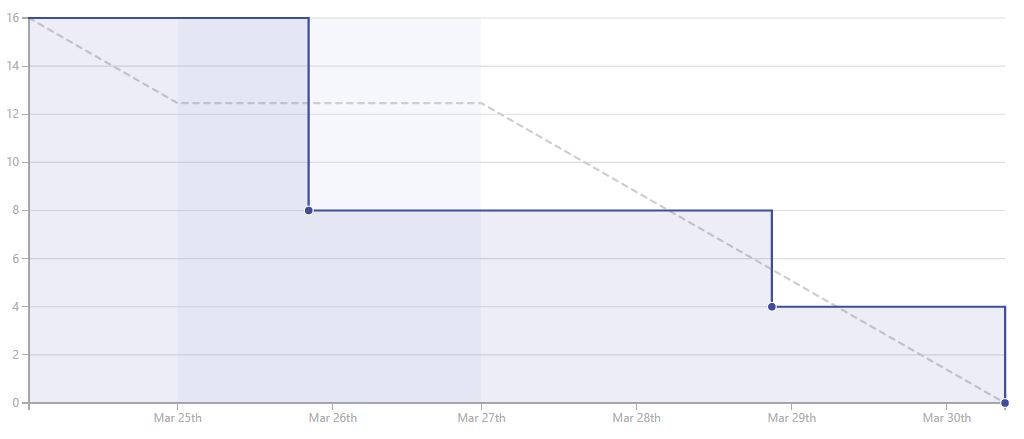
\includegraphics[width=0.99\textwidth]{sprint_7}
\caption{Burndown del \textit{sprint} 7}
\label{fig:A.1.8}
\end{figure}


\subsection{\textit{Sprint} 8}
Estas son las tareas a realizar durante este \textit{sprint} 8:

\begin{itemize}
	\item Implementar la funcionalidad de obtención de imágenes en el etiquetador de imágenes, o \textit{Widget}.
	\item Mejorar la interfaz del etiquetador de imágenes.
	\item Crear un primer prototipo de interfaz de usuario.
\end{itemize}

Durante este \textit{sprint} se realizó un primer prototipo de interfaz de  usuario. Partiendo de este prototipo, se mejoró la interfaz del etiquetador de imágenes. Consiguiendo, así, una interfaz adecuada para el cliente. Además, se implemento la funcionalidad que nos permitiría obtener una imágen resultante de cada etiqueta realizada en las distintas imágenes.

A continuación, en la figura \ref{fig:A.1.9}, se muestra el diagrama \textit{burndown} de este \textit{sprint}.

\begin{figure}
\centering
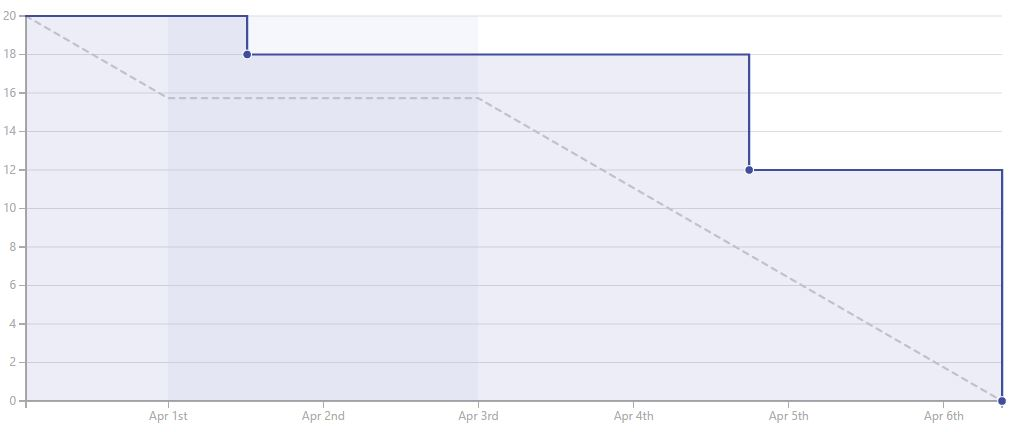
\includegraphics[width=0.99\textwidth]{sprint_8}
\caption{Burndown del \textit{sprint} 8}
\label{fig:A.1.9}
\end{figure}

\subsection{\textit{Sprint} 9}

Este \textit{sprint} tendrá una duración de dos semanas. Debido  a la carga de trabajo asociada a este \textit{sprint} y al ser días no lectivos por las vacaciones de Semana Santa. 

Estas son las tareas a realizar durante este \textit{sprint} 9:

\begin{itemize}
	\item Añadir un texto a cada etiqueta que realizamos en una imagen.
	\item Añadir notificaciones al usuario en la carga y guardado de imágenes.
	\item Guardar las coordenadas de las etiquetas de cada imagen.
	\item Cargar las etiquetas de una imagen que haya sido previamente etiquetada.
	\item Controlar que el usuario no cree etiquetas en el SVG pero fuera de la imagen.
	\item Añadir la posibilidad de eliminar etiquetas previamente realizadas.
	\item Añadir un botón que permita guardar imágenes como negativos.
	\item Corregir los \textit{notebooks} creados para la técnica \textit{Bag of Words}.
\end{itemize}

Durante este \textit{sprint} se completaron todas las tareas asignadas, excepto la corrección de los \textit{notebooks} para la técnica \textit{Bag of Words}. Los cuales no se revisaron porque no se utilizarían por el momento.

A continuación, en la figura \ref{fig:A.1.10}, se muestra el diagrama \textit{burndown} de este \textit{sprint}.

\begin{figure}
\centering
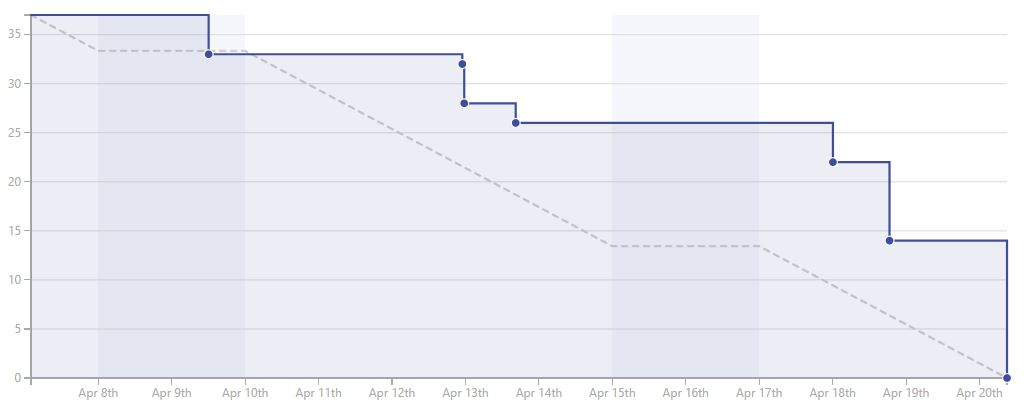
\includegraphics[width=0.99\textwidth]{sprint_9}
\caption{Burndown del \textit{sprint} 9}
\label{fig:A.1.10}
\end{figure}


\subsection{\textit{Sprint} 10}

Estas son las tareas a realizar durante este \textit{sprint} 10:

\begin{itemize}
	\item Tratar de reentrenar a \textit{YOLO}.
	\item Corregir errores en la carga de etiquetas.
	\item Mejorar la interfaz del etiquetador de imágenes.
	\item Documentación: manual de usuario del etiquetador de imágenes.
	\item Documentación: diseño(prototipo).
\end{itemize}

Durante este \textit{sprint} se comenzaron las pruebas con el detector automático de objetos, para su futura adaptación a la detección de fitolitos. Además, se trataron de solucionar algunos errores presentes en el etiquetador. Y, finalmente, se documentó en la medida de lo posible el manual del etiquetador. Tratando de facilitar su uso por parte de los usuarios, en breves momentos.

A continuación, en la figura \ref{fig:A.1.11}, se muestra el diagrama \textit{burndown} de este \textit{sprint}.

\begin{figure}
\centering
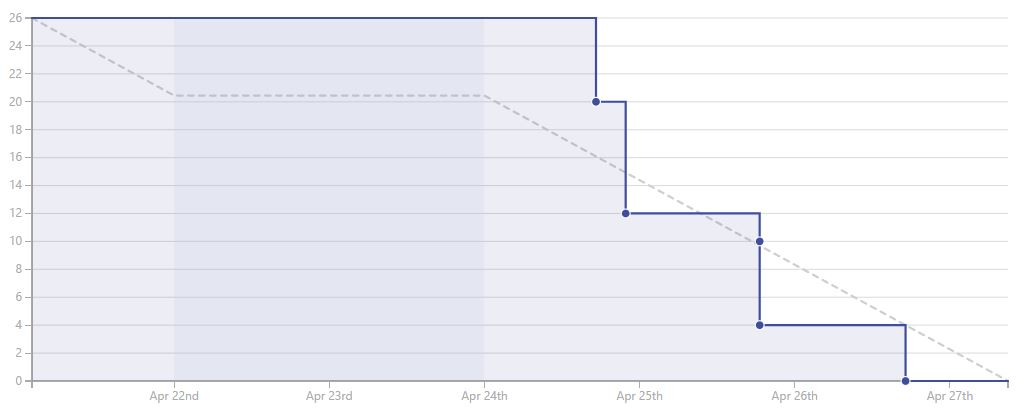
\includegraphics[width=0.99\textwidth]{sprint_10}
\caption{Burndown del \textit{sprint} 10}
\label{fig:A.1.11}
\end{figure}

\subsection{\textit{Sprint} 11}

Estas son las tareas a realizar durante este \textit{sprint} 11:

\begin{itemize}
	\item Documentación: aspectos relevantes
	\item Documentación: conceptos \textit{YOLO} y \textit{BoW}
	\item Documentación: técnicas y herramientas.
	\item Documentación: manual del programador.
	\item Poner correctamente los separadores de archivo en Linux Y Windows.
	\item Crear script para la lectura de las coordenadas desde \textit{YOLO}.
	\item Documentación: \textit{README}.
\end{itemize}

Durante este \textit{sprint}, principalmente, se trato de documentar algunos de los aspectos de la memoria. Y, por último, se creó un \textit{script} para la lectura y conversión de las coordenadas para el entrenamiento de \textit{YOLO}.

A continuación, en la figura \ref{fig:A.1.12}, se muestra el diagrama \textit{burndown} de este \textit{sprint}.

\begin{figure}
\centering
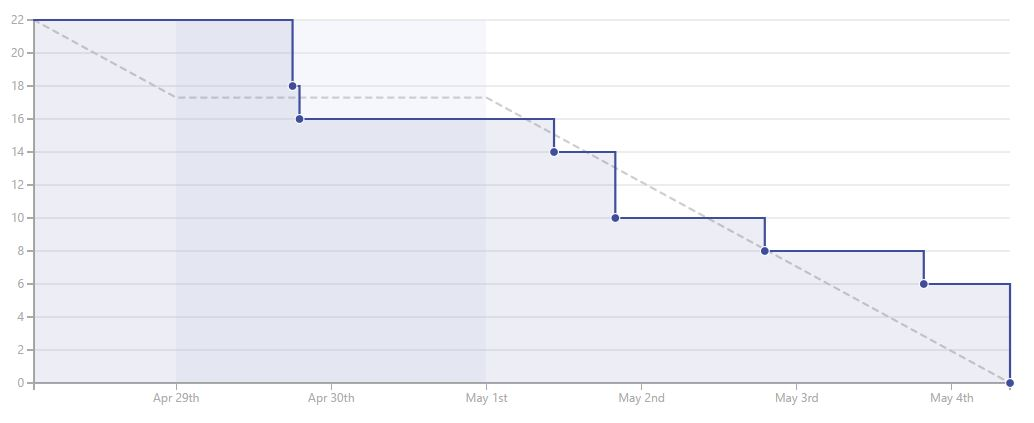
\includegraphics[width=0.99\textwidth]{sprint_11}
\caption{Burndown del \textit{sprint} 11}
\label{fig:A.1.12}
\end{figure}

\subsection{\textit{Sprint} 12}

Estas son las tareas a realizar durante este \textit{sprint} 12:

\begin{itemize}
	\item \textit{Data augmentation}: rotar imágenes y coordenadas en ángulos de 90 grados.
	\item \textit{Data augmentation}: espejar imágenes.
	\item \textit{Data augmentation}: aplicar ruidos a las imágenes.
	\item \textit{Data augmentation}: realizar cambios de tamaño en las imágenes.
	\item Documentación: introducción.
	\item Documentación: objetivos del proyecto.
	\item Documentación: trabajos relacionados.
	\item Documentación: Documentación: diseño arquitectónico y procedimental.
\end{itemize}

Durante este \textit{sprint} se trato de continuar escribiendo algunos de los aspectos todavía no documentados hasta el momento. Y se creo una herramienta para la aplicación de técnicas de \textit{data augmentation} sobre un conjunto de imágenes. Además, la última de las tareas planteadas para este \textit{sprint} fue completada en un sprint más adelante por ser muy subestimada en cuanto al esfuerzo requerido.

A continuación, en la figura \ref{fig:A.1.13}, se muestra el diagrama \textit{burndown} de este \textit{sprint}.

\begin{figure}
\centering
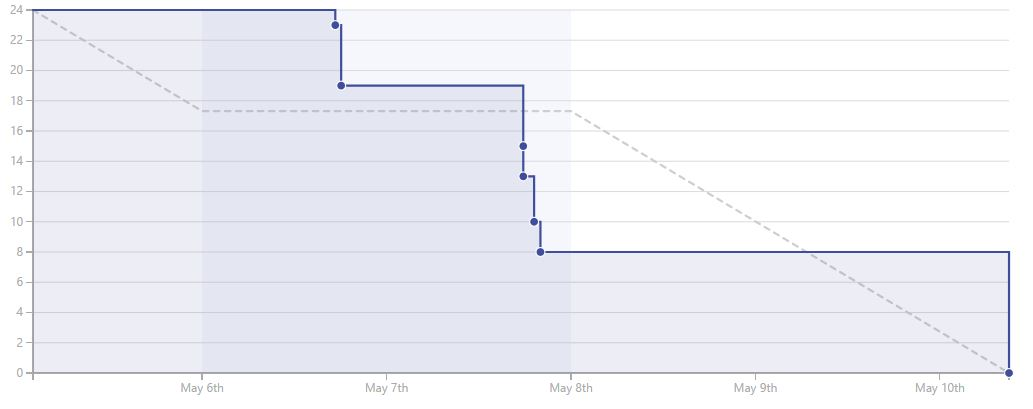
\includegraphics[width=0.99\textwidth]{sprint_12}
\caption{Burndown del \textit{sprint} 12}
\label{fig:A.1.13}
\end{figure}

\subsection{\textit{Sprint} 13}

Estas son las tareas a realizar durante este \textit{sprint} 13:

\begin{itemize}
	\item \textit{Data augmentation}: generador de imágenes.
	\item \textit{Data augmentation}: aplicar filtros en las imágenes (clarecer,oscurecer).
	\item Entrenar por primera vez a YOLO con un primer dataset de fitolitos.
\end{itemize}

Durante este \textit{sprint} se finalizo el generador de imágenes que aplicaba las técnicas de \textit{data augmentation}, implementadas durante el \textit{sprint} anterior, para generar un conjunto de imágenes mucho mayor. Y, además, dado que nuestros clientes nos enviaron un conjunto de imágenes etiquetadas de fitolitos, comenzamos con los primeros entrenamientos a \textit{YOLO}.

A continuación, en la figura \ref{fig:A.1.14}, se muestra el diagrama \textit{burndown} de este \textit{sprint}.

\begin{figure}
\centering
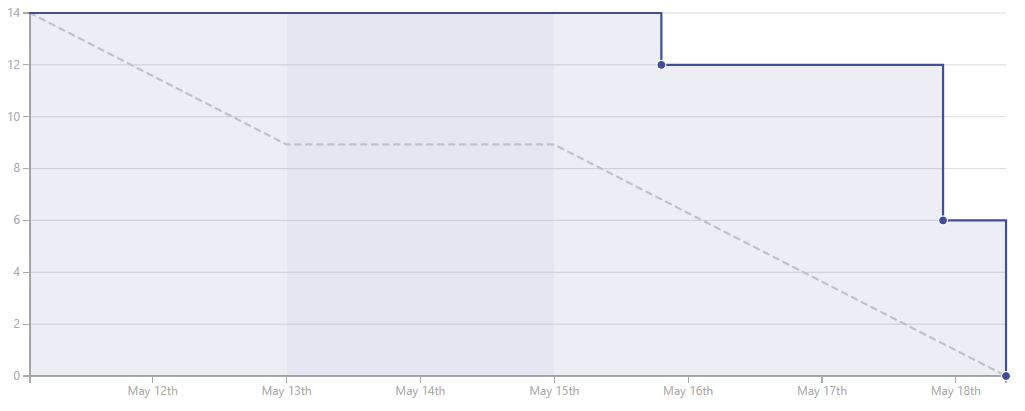
\includegraphics[width=0.99\textwidth]{sprint_13}
\caption{Burndown del \textit{sprint} 13}
\label{fig:A.1.14}
\end{figure}

\subsection{\textit{Sprint} 14}

Estas son las tareas a realizar durante este \textit{sprint} 14:

\begin{itemize}
	\item Correcciones menores en fichero \textit{README}.
	\item Evaluar los resultados de \textit{YOLO} con un primer dataset.
	\item Entrenar a YOLO con el dataset aplicando \textit{data augmentation}.
\end{itemize}

Durante este \textit{sprint} se entrenó a YOLO, con un dataset de un tamaño mayor. Además, se completaron otras tareas pendientes de las semanas anteriores, relativas a la documentación y a la evaluación del modelo generado por el entrenamiento.

A continuación, en la figura \ref{fig:A.1.15}, se muestra el diagrama \textit{burndown} de este \textit{sprint}.

\begin{figure}
\centering
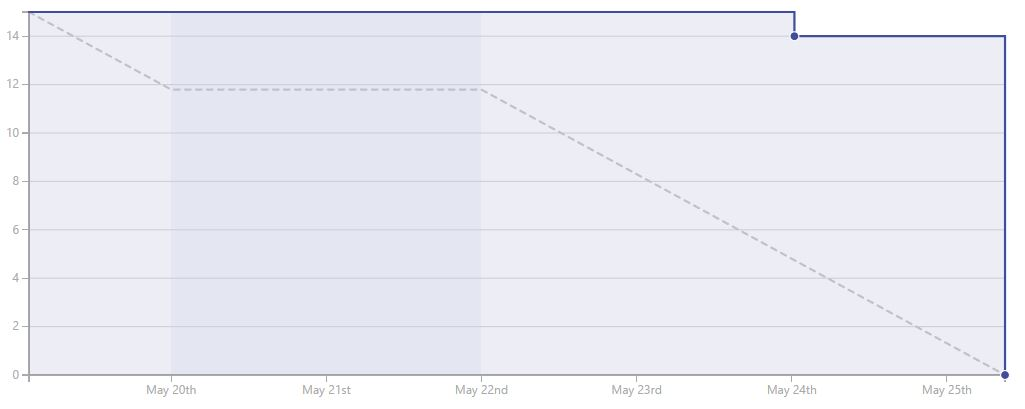
\includegraphics[width=0.99\textwidth]{sprint_14}
\caption{Burndown del \textit{sprint} 14}
\label{fig:A.1.15}
\end{figure}

\subsection{\textit{Sprint} 15}

Estas son las tareas a realizar durante este \textit{sprint} 15:

\begin{itemize}
	\item Documentación: lineas futuras.
	\item Reetiquetar un único tipo de fitolitos.
	\item Documentación: completar el anexo de planificación del proyecto.
	\item Documentación: completar los aspectos restantes del anexo de diseño.
	\item Documentación: Preparar el anexo de requisitos.
	\item Entrenar el clasificador con los fitolitos reetiquetados.
\end{itemize}

Durante esta semana, principalmente, se trato de continuar con aspectos de documentación. Y, a su vez, se continuo entrenando a \textit{YOLO} con el fin de conseguir algún resultado. 

A continuación, en la figura \ref{fig:A.1.16}, se muestra el diagrama \textit{burndown} de este \textit{sprint}.

\begin{figure}
\centering
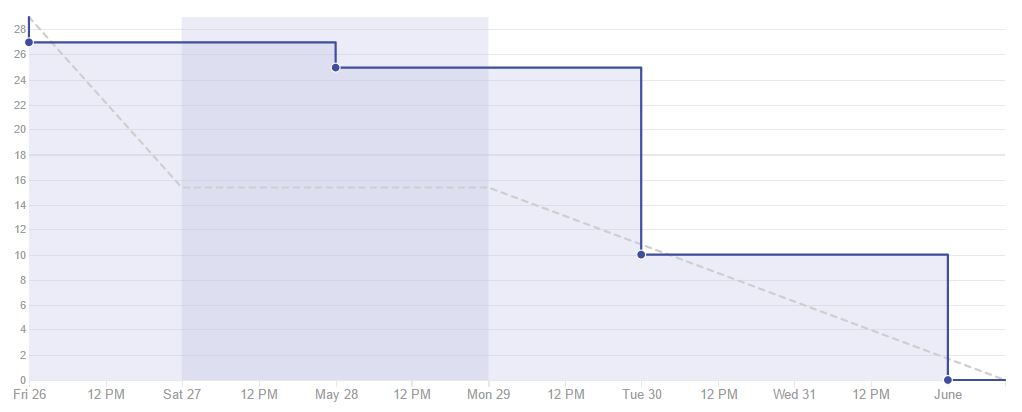
\includegraphics[width=0.99\textwidth]{sprint_15}
\caption{Burndown del \textit{sprint} 15}
\label{fig:A.1.16}
\end{figure}

\subsection{\textit{Sprint} 16}

Estas son las tareas a realizar durante este \textit{sprint} 16:

\begin{itemize}
	\item Documentación: Complejidad de la tarea.
	\item Unificar separadores en todos los fuentes.
	\item Documentación: conceptos teóricos restantes.
	\item Desarrollar teses para los distintos módulos.
\end{itemize}

Durante esta semana se unificaron los separadores del sistemas operativo, se documento y se realizaron teses para los módulos más relevantes del sistema.

A continuación, en la figura \ref{fig:A.1.17}, se muestra el diagrama \textit{burndown} de este \textit{sprint}.

\begin{figure}
\centering
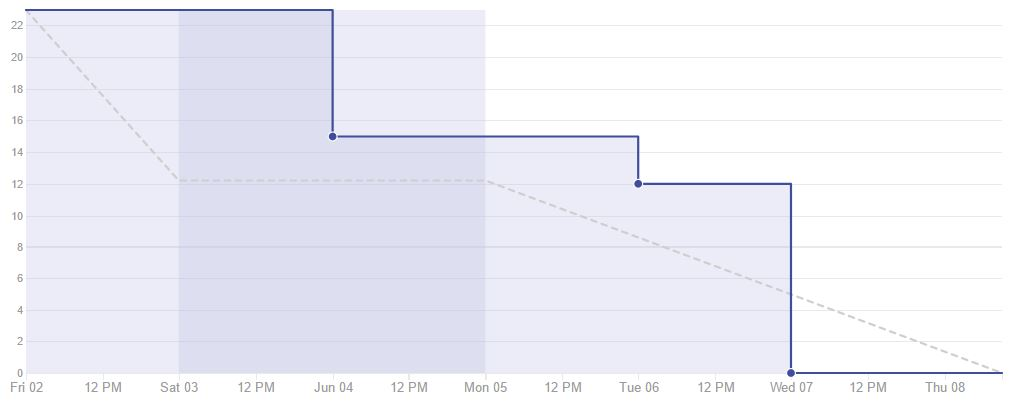
\includegraphics[width=0.99\textwidth]{sprint_16}
\caption{Burndown del \textit{sprint} 16}
\label{fig:A.1.17}
\end{figure}

\subsection{\textit{Sprint} 17}

Estas son las tareas a realizar durante este \textit{sprint} 17:

\begin{itemize}
	\item Añadir la funcionalidad de clasificar fitolitos.
\end{itemize}

Durante esta semana se volvió al enfoque mediante clasificadores. Principalmente, se trato de encontrar las distintas opciones para la clasificación de fitolitos y evaluar los resultados. Para, más tarde, aplicarlo a la detección de estos mediante ventana deslizante.

A continuación, en la figura \ref{fig:A.1.18}, se muestra el diagrama \textit{burndown} de este \textit{sprint}.

\begin{figure}
\centering
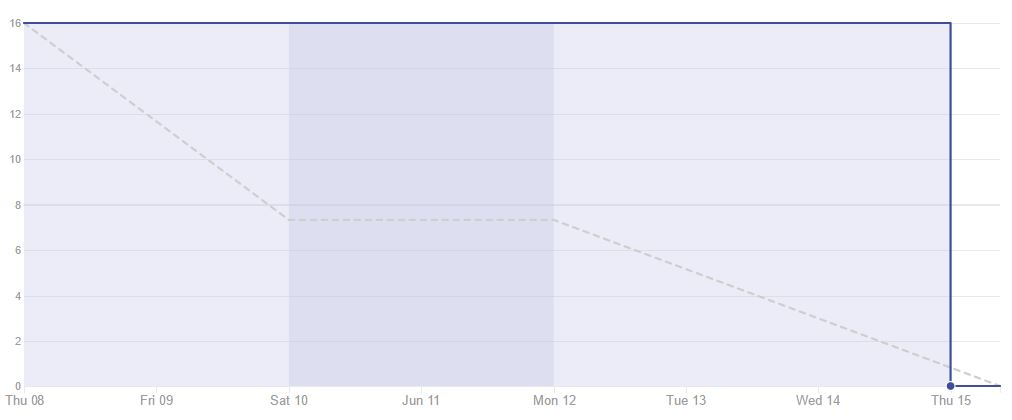
\includegraphics[width=0.99\textwidth]{sprint_17}
\caption{Burndown del \textit{sprint} 17}
\label{fig:A.1.18}
\end{figure}

\subsection{\textit{Sprint} 18}

Estas son las tareas a realizar durante este \textit{sprint} 18:

\begin{itemize}
	\item Hallar el mejor clasificador posible.
	\item Aplicar la ventana deslizante a las imágenes de fitolitos.
\end{itemize}

Durante esta semana se obtuvo el clasificador que mejor se adaptaba a la problemática mediante un \textit{script} que evaluaba las distintas opciones. Y, finalmente, se aplico a la detección de fitolitos en imágenes.

A continuación, en la figura \ref{fig:A.1.19}, se muestra el diagrama \textit{burndown} de este \textit{sprint}.

\begin{figure}
\centering
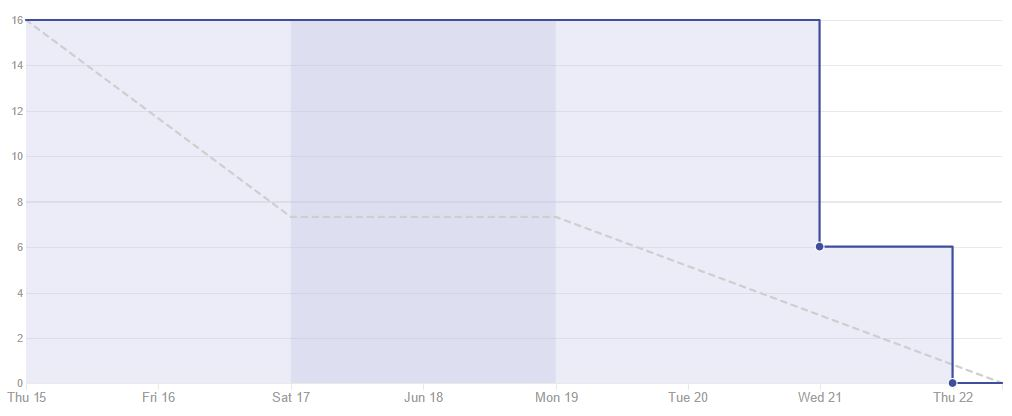
\includegraphics[width=0.99\textwidth]{sprint_18}
\caption{Burndown del \textit{sprint} 18}
\label{fig:A.1.19}
\end{figure}

\section{Estudio de viabilidad}

\subsection{Viabilidad económica}
En esta sección se realiza un análisis de los costes económicos que hubiera supuesto el desarrollo de este proyecto en un entorno empresarial.

\subsubsection{Coste del personal}
Este proyecto ha sido desarrollado por un único desarrollador a tiempo parcial. En la tabla \ref{tabla:costespersonales} muestro el desglose de los costes ocasionados por el salario que hubiese recibido en una situación real.

\tablaSmallSinColores{Costes de personal}{p{4.5cm} p{.25cm} p{2.5cm}}{costespersonales}{
  \multicolumn{3}{p{6cm}}{\textbf{Costes de personal}} \\
 }
 {
  Salario mensual neto  & 1500\euro{} \\
  Retención IRPF (15\%) & \euro{} \\
  Seguridad social (29,9\%) & \euro{} \\
  Salario mensual bruto  & \euro{} \\\hline
  Salario total(4 meses)  & \euro{} \\
  }

\subsubsection{Coste del \textit{software} y \textit{hardware}}



\subsubsection{Costes totales}



\subsection{Viabilidad legal}

En este apartado enuncio las distintas librerías utilizadas junto a sus licencias, en todos sus casos de código abierto. Véase la tabla \ref{tabla:licencias}. Si se desea indagar más sobre las distintas librerías se recomienda ver la sección de herramientas y técnicas dentro de la memoria.
 
  \begin{table}
  \begin{center}
   \begin{tabular}{p{3.5cm} p{1.5cm} p{2.5cm}}
    \toprule
    \textbf{Librería} & \textbf{Versión} & \textbf{Licencia} \\
    \otoprule
    Numpy & 1.12 & BSD \\
    scikit-learn & 0.18 & BSD \\
    scikit-image & 0.13 & BSD \\
    Matplotlib & 1.12 & PSF \\
    Jupyter Notebook & 1 & BSD \\
    Jupyter Dashboards & 0.6 & BSD \\
	Ipython File Upload & 0.1.2 & MIT \\
	darkflow & 0 & GPL 3 \\
    \bottomrule
   \end{tabular}
   \caption{Licencias de las librerías}
   \label{tabla:licencias}
  \end{center}
 \end{table}
 
 Finalmente, este proyecto esta publicado bajo la licencia \textit{BSD 3-clause} con la que se permite un libre uso, modificación, distribución y uso privado de este. Sin embargo, con la condición de que el código debe ser suministrado en todas las ocasiones junto a la licencia que expone las distintas garantías de uso. Para finalizar, esta licencia introduce una muy limitada responsabilidad sobre la utilización de este proyecto y ningún tipo de garantía.
